% Options for packages loaded elsewhere
\PassOptionsToPackage{unicode}{hyperref}
\PassOptionsToPackage{hyphens}{url}
%
\documentclass[
]{article}
\usepackage{amsmath,amssymb}
\usepackage{iftex}
\ifPDFTeX
  \usepackage[T1]{fontenc}
  \usepackage[utf8]{inputenc}
  \usepackage{textcomp} % provide euro and other symbols
\else % if luatex or xetex
  \usepackage{unicode-math} % this also loads fontspec
  \defaultfontfeatures{Scale=MatchLowercase}
  \defaultfontfeatures[\rmfamily]{Ligatures=TeX,Scale=1}
\fi
\usepackage{lmodern}
\ifPDFTeX\else
  % xetex/luatex font selection
\fi
% Use upquote if available, for straight quotes in verbatim environments
\IfFileExists{upquote.sty}{\usepackage{upquote}}{}
\IfFileExists{microtype.sty}{% use microtype if available
  \usepackage[]{microtype}
  \UseMicrotypeSet[protrusion]{basicmath} % disable protrusion for tt fonts
}{}
\makeatletter
\@ifundefined{KOMAClassName}{% if non-KOMA class
  \IfFileExists{parskip.sty}{%
    \usepackage{parskip}
  }{% else
    \setlength{\parindent}{0pt}
    \setlength{\parskip}{6pt plus 2pt minus 1pt}}
}{% if KOMA class
  \KOMAoptions{parskip=half}}
\makeatother
\usepackage{xcolor}
\usepackage{graphicx}
\makeatletter
\def\maxwidth{\ifdim\Gin@nat@width>\linewidth\linewidth\else\Gin@nat@width\fi}
\def\maxheight{\ifdim\Gin@nat@height>\textheight\textheight\else\Gin@nat@height\fi}
\makeatother
% Scale images if necessary, so that they will not overflow the page
% margins by default, and it is still possible to overwrite the defaults
% using explicit options in \includegraphics[width, height, ...]{}
\setkeys{Gin}{width=\maxwidth,height=\maxheight,keepaspectratio}
% Set default figure placement to htbp
\makeatletter
\def\fps@figure{htbp}
\makeatother
\setlength{\emergencystretch}{3em} % prevent overfull lines
\providecommand{\tightlist}{%
  \setlength{\itemsep}{0pt}\setlength{\parskip}{0pt}}
\setcounter{secnumdepth}{-\maxdimen} % remove section numbering
\ifLuaTeX
\usepackage[bidi=basic]{babel}
\else
\usepackage[bidi=default]{babel}
\fi
\babelprovide[main,import]{italian}
% get rid of language-specific shorthands (see #6817):
\let\LanguageShortHands\languageshorthands
\def\languageshorthands#1{}
\usepackage{cancel}
\usepackage{steinmetz}
\usepackage{derivative}
\usepackage{tabularray}
\usepackage{mathtools}
\usepackage{siunitx}
\usepackage{geometry}
\usepackage{array}
\usepackage{hhline}
    \geometry{
        a4paper,
        total={170mm,257mm},
        left=20mm,
        top=20mm,
    }
\ifLuaTeX
  \usepackage{selnolig}  % disable illegal ligatures
\fi
\usepackage{bookmark}
\IfFileExists{xurl.sty}{\usepackage{xurl}}{} % add URL line breaks if available
\urlstyle{same}
\hypersetup{
  pdflang={it},
  hidelinks,
  pdfcreator={LaTeX via pandoc}}

\author{}
\date{}

\begin{document}

{
\setcounter{tocdepth}{3}
\tableofcontents
}
\newpage

\section{Capitolo 1 Dispositivi
elettronici}\label{capitolo-1-dispositivi-elettronici}

I dispositivi dei circuiti integrati sono fatti principalmente in
silicio (S) o in germanio (Ge) o in qualche lega come GaAs, GaN, InP,
SiC, ovvero materiali con 3/4/5 elettroni nell'orbitale esterno. Questi
materiali sono chiamati semiconduttori.

Accanto ai semiconduttori servono altri materiali capaci di dotarli di
conduttività selettiva: in pratica prendiamo un semiconduttore (ad
esempio il silicio) e inseriamo all'interno del suo reticolo cristallino
degli atomi di un elemento drogante. L'elemento drogante viene inserito
con un rapporto dell'ordine di \(1:10{}^{10}\) (questo è il caso di un
drogaggio pesante, se no è ancora minore la quantità di elemento
drogante).

Il vantaggio di inserire un elemento drogante all'interno del reticolo
cristallino è che gli altri atomi lo vedono come uno di loro solo con un
elettrone in più o in meno. Il drogaggio può essere \textbf{di tipo P}
se l'elemento drogante ha un elettrone in meno rispetto al
semiconduttore (ad esempio se drogo il silicio con il boro), oppure
\textbf{di tipo N} se l'elemento drogante ha un elettrone in più (ad
esempio se drogo il silicio con il fosforo). Nel primo caso ottengo
delle lacune, nel secondo degli elettroni in eccesso.

\subsection{1.1 Giunzione P-N}\label{giunzione-p-n}

Una giunzione P-N e formata da una sezione del semiconduttore drogata
con un drogaggio P (con una percentuale \(N_{a}\), n.~accettori) e
un'altra sezione drogata con un drogaggio N (con una percentuale
\(N_{d}\), n.~donatori).

\begin{figure}
\centering
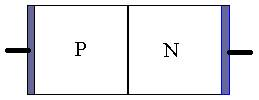
\includegraphics[width=\textwidth,height=0.05\textheight]{immagini/0.jpg}
\caption{Giunzione P-N}
\end{figure}

Queste due sezioni devono essere adiacenti, così che gli elettroni
possano migrare dalla parte drogata N a quella drogata P per formare al
centro una regione detta \textbf{regione di svuotamento} (dove ho
riprodotto il reticolo cristallino classico).

\begin{figure}
\centering
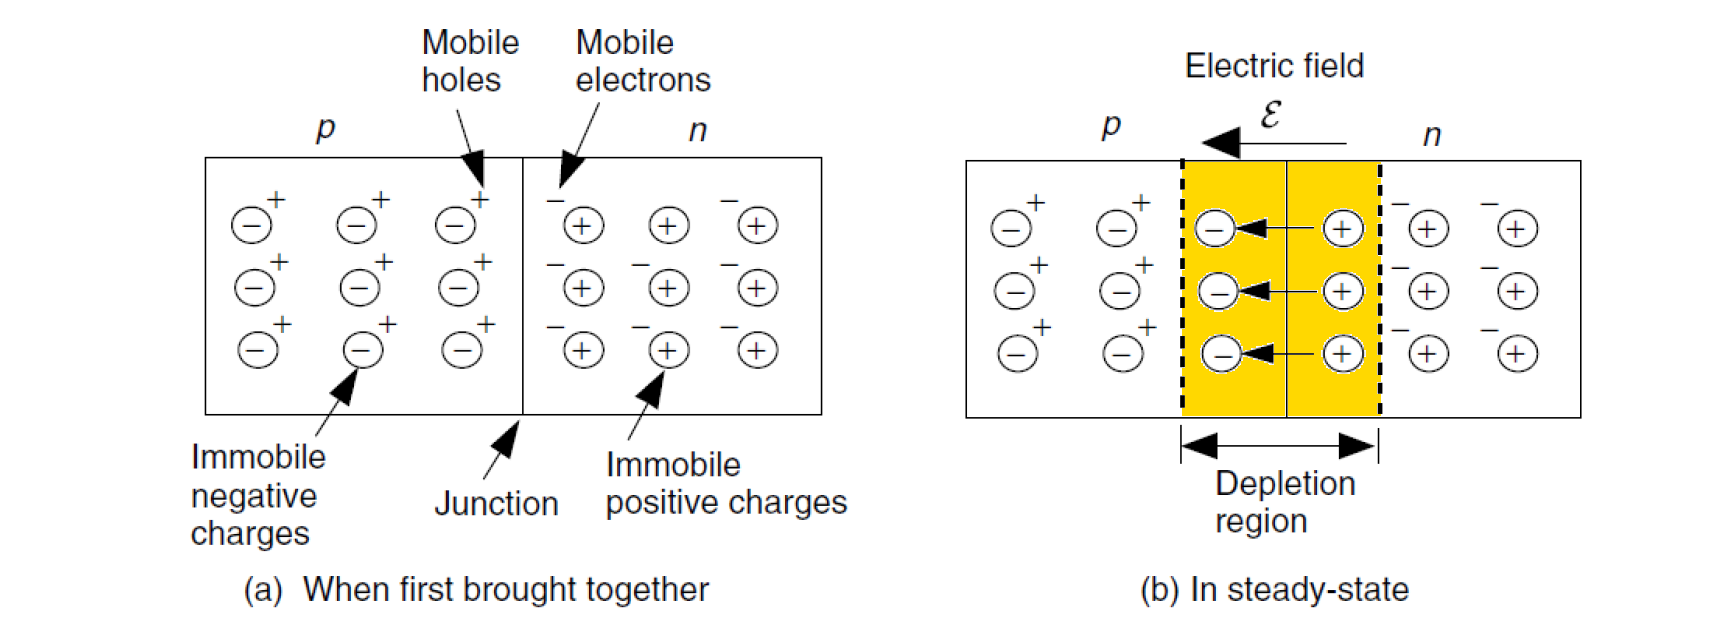
\includegraphics[width=0.68\textwidth,height=\textheight]{immagini/1.png}
\caption{Regione di svuotamento}
\end{figure}

Lo scopo della regione di svuotamento è impedire che altre cariche
negative di N possano fluire in P. La quantità di carica presente su
ciascuna delle ''sezioni''della regione di svuotamento dev'essere
uguale, tuttavia le dimensioni delle sezioni può essere diversa e
influenzata dalla percentuale di drogante.

\begin{figure}
\centering
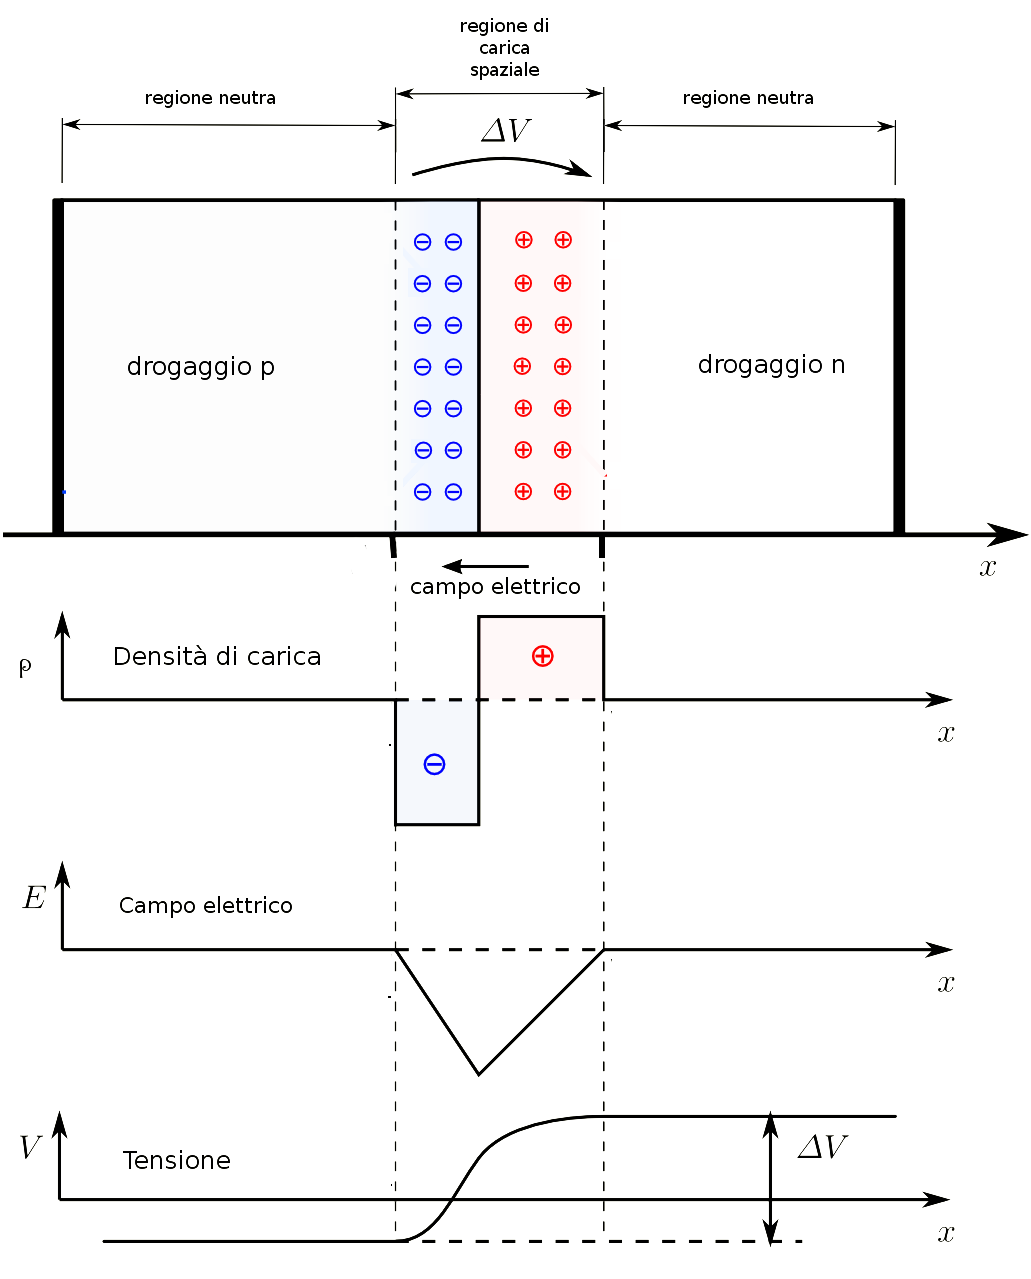
\includegraphics[width=\textwidth,height=0.35\textheight]{immagini/2.png}
\caption{``Grafici relativi alla regione di svuotamento''}
\end{figure}

Affinché un elettrone ``salti'' la barriera deve esserci un buon motivo
e questo può essere dato fornendogli energia. La giunzione P-N permette
il passaggio selettivo di cariche.

La giunzione P-N può essere utilizzata per creare un \textbf{diodo P-N}.
Tale diodo prevede l'applicazione di potenziale positivo dal lato P e
negativo dal lato N in modo tale da neutralizzare le lacune in P o da
fornire elettroni alla parte della regione di svuotamento di N.

Le componenti elettroniche cambiano stato \emph{molto} velocemente.

Gli elettroni che fluiscono nella p-region sono detti \textbf{minority
carries} (e non fanno parte del reticolo). Se faccio passare la corrente
al contrario (quindi metto il potenziale positivo dal lato N) impedisco
il passaggio di corrente, estendo la regione di svuotamento e incremento
il campo elettrico fino ad un punto detto \textbf{di breakdown} dove la
corrente fluisce normalmente.

Se il diodo è scaldato funziona meglio.

\subsubsection{1.1.1 Formule}\label{formule}

\textbf{Forward bias}

\[I_{d}=I_{0}(e^{\frac{V_{d}}{nV_{t}}}\ -1)\]

\(I_{0}\) è un valore tipo \(10^{-10}\), \(V_{d}\) e la ddp tra i capi
del diodo, \(nV_{t}\) sarà il \emph{potenziale nativo dei diodi}
\((0.7V)\)

\begin{figure}
\centering
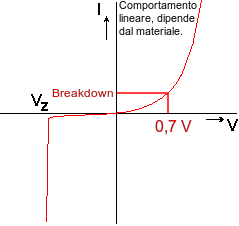
\includegraphics[width=0.3\textwidth,height=\textheight]{immagini/3.png}
\caption{Grafico che spiega a grandi linee il comportamento di un diodo
P-N al variare della differenza di potenziale}
\end{figure}

\subsection{1.2 Diodi particolari}\label{diodi-particolari}

\subsubsection{1.2.1 Fotodiodi}\label{fotodiodi}

\begin{figure}
\centering
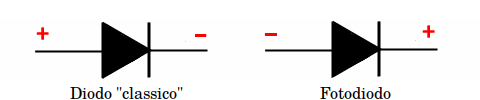
\includegraphics[width=0.5\textwidth,height=\textheight]{immagini/4.png}
\caption{I fotodiodi sono polarizzati inversamente}
\end{figure}

I fotodiodi sono diodi la cui giunzione o è scoperta o è incapsulata in
un materiale trasparente.

Se la giunzione è colpita da un fascio di protoni (che ha una certa
energia) può darsi che qualche fotone ``porti via'' al reticolo
cristallino un elettrone così da creare una nuova coppia
elettrone-lacuna e far passare corrente.

La corrente che scorre nel diodo non dipende dalla tensione applicata ai
suoi capi ma solo dal flusso luminoso che colpisce la giunzione.

\subsubsection{1.2.2 Formule}\label{formule-1}

\[
I_d = k \cdot E_{L}
\]

FIGURA

\(k\) è una costante che ci dice il produttore del diodo, \(E_L\) è il
flusso luminoso (in \(W /m^2\)) che incide sul fotodiodo.

\subsubsection{Led}\label{led}

I led (light emitting diode) sono anch'essi diodi la cui giunzione è
impacchettata in un involucro trasparente. La loro barriera non si trova
a \(0.7V\) ma bensì a \textbf{\(1.5V\)}.

\begin{align*}
E&=h\cdot\nu\ (E = \text{energia emessa}, h = \text{costante di Plank}, \nu = \text{frequenza
dell'onda luminosa})\\
\nu&=\frac{E}{h}\ \Longrightarrow\ \nu\propto E \\
\lambda\nu&=c, \quad \lambda\propto\frac{1}{E}
\end{align*}

Colori diversi di luce richiedono differenze di potenziale diverse: si
va da un 1.5V per un led rosso (possiamo avere anche meno con un led IR)
a un 3.0V per un led viola (e poi sale nel caso dei led UV).

I led bianchi sono led ultravioletti ricoperti di una miscela di fosfori
(ne esistono di tre tipi: rossi, blu e verdi) in una certa proporzione
tale da simulare la luce calda, quella ``neutra'' o quella fredda.

La luce viene emessa perché gli elettroni che si trovano ad uno stato
energetico più alto ``saltano'' verso uno stato più basso e perdono
energia in forma luminosa.

\subsubsection{Diodi Schottky}\label{diodi-schottky}

I diodi Schottky sono diodi in cui la parte P è sostituita con un
metallo (solitamente alluminio). Nella parte metallica non si può creare
la regione di svuotamento. La tensione di soglia è circa 0.3-0.4V. I
vantaggi di questo diodo sono che da freddo si comporta bene come un
diodo ``normale'' scaldato, si spegne velocemente e passa rapidamente da
conduzione diretta a conduzione inversa. \newline Viene utilizzato dove
e un problema avere 0.7V di caduta, quindi tipo nei circuiti di potenza
o nei circuiti logici.

\begin{figure}
\centering
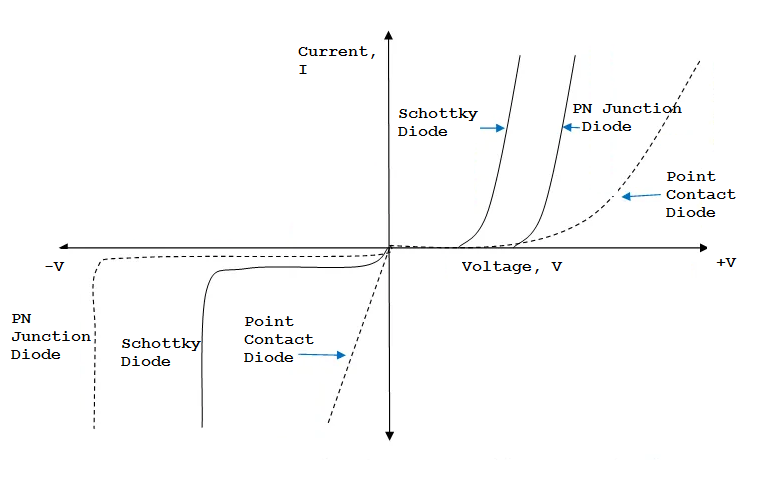
\includegraphics[width=0.5\textwidth,height=\textheight]{immagini/6.png}
\caption{Grafico che spiega a grandi linee il comportamento di un diodo
Schottky in confronto ad un non Schottky}
\end{figure}

\subsection{1.3 Leggi di Kirchoff}\label{leggi-di-kirchoff}

\begin{enumerate}
\def\labelenumi{\arabic{enumi}.}
\tightlist
\item
  La somma delle correnti in un nodo è 0
\item
  La somma delle tensioni lungo un percorso chiuso è 0
\end{enumerate}

\subsection{1.4 BJT: giunzione n-p-n (transistor
bipolare)}\label{bjt-giunzione-n-p-n-transistor-bipolare}

\begin{figure}
\centering
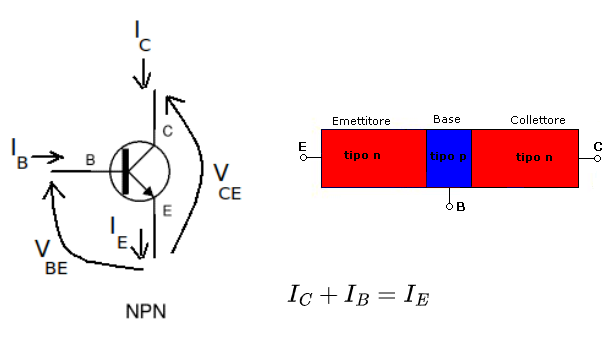
\includegraphics[width=0.5\textwidth,height=\textheight]{immagini/7.png}
\caption{Schema di un transistor bipolare}
\end{figure}

N.B.: la base è molto stretta così che la corrente possa passare senza
problemi.

Ci sono 4 regioni di funzionamento:

\begin{enumerate}
\def\labelenumi{\arabic{enumi}.}
\tightlist
\item
  cutoff (quando il transistor e spento)
\item
  attiva diretta
\item
  saturazione
\item
  attiva inversa
\end{enumerate}

\begin{itemize}
\item
  \textbf{Cutoff}: Il dispositivo è spento (come se fosse un
  interruttore aperto), perciò
  \[V_{be}\ {\rm e}\ V_{bc}<V_{th},\ I_{b}=0,\ I_{c}=0\]
\item
  \textbf{Attiva diretta}: Si ha quando \(V_{be}>V_{th}\) e quindi
  \(I_{b}>0,\ I_{c}=h_{fe}I_{b}\), (\(h_{fe}\) è una funzione di
  guadagno). Figura 1.8
\item
  \textbf{Saturazione} \begin{gather*}
  V_{be}>V_{th},\ V_{ce}<V_{ce-sat}\ \Longrightarrow\ V_{bc}>V_{th} \\
  I_{b}>0,I_{c}<h_{fe}I_{b}
  \end{gather*}
\item
  \textbf{Attiva inversa} \begin{gather*}
  V_{be}<0,\ V_{bc}>V_{th} \\
  I_{e} =-I_{b}\ (\text{il gain è }\leq 1)
  \end{gather*}
\end{itemize}

\begin{figure}
\centering
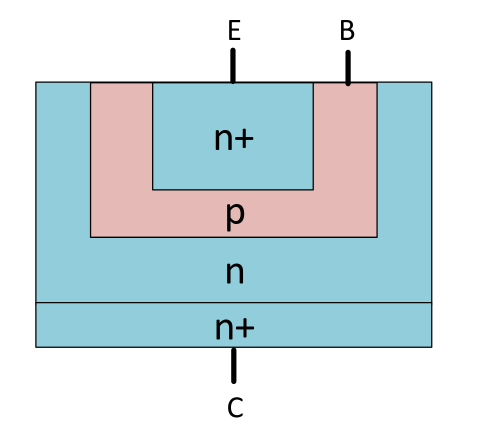
\includegraphics[width=0.2\textwidth,height=\textheight]{immagini/9.png}
\caption{Schema fisico di un BJT}
\end{figure}

\subsection{1.5 Sonda 10x}\label{sonda-10x}

\begin{figure}
\centering
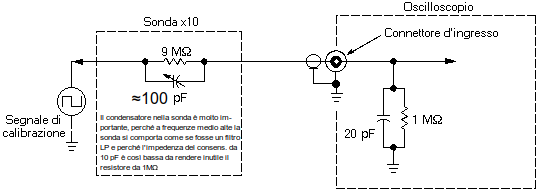
\includegraphics[width=0.6\textwidth,height=\textheight]{immagini/10.png}
\caption{Schema di una sonda 10x}
\end{figure}

\emph{Bandwidth limit}: un tastino sull'oscilloscopio che taglia le
frequenze sopra i 20MHz.\newpage

\subsection{1.6 Diodo Zener}\label{diodo-zener}

Figure 1.11: Schema di un diodo zener Questo tipo di diodo lavora in
breakdown. Se lo metto in polarizzazione diretta funziona come un diodo
normale, se però lo metto in polarizzazione inversa faccio si che la
tensione di breakdown sia molto precisa e quindi se \(V_{G}<V_{Z}\) non
succede nulla (\(V_{G}=V_{0}\)). Se invece \(V_{G}\geq V_{Z}\) allora il
diodo va in breakdown e inizia a scorrere corrente in esso. Di preciso
scorre \(V_{0}=V_{Z}\) (e quindi ho una tensione in uscita
stabilizzata).

Nel circuito in figura 1.11 la resistenza e importante perché se non ci
fosse avrei \(\frac{V_{G}-V_{i}}{R}=i_{r}\) ma \(R\to 0\) e quindi
\(i_{r}\to\infty\).

\subsection{1.7 BJT pnp}\label{bjt-pnp}

Questo dispositivo è complementare al npn: le equazioni sono le medesime
ma il verso delle correnti e delle tensioni è inverso.

Figure 1.12: Schema di un transistor pnp

Rispetto al npn, il pnp ha un gain minore e quindi funziona peggio (per
questo motivo, quando e possibile, si utilizzano gli npn), ovvero scorre
meno corrente (ha un'efficienza di circa la metà degli elettroni).

\subsection{1.8 Fototransistor}\label{fototransistor}

La corrente di base viene generata quando è esposto alla luce, per il
resto è un transistor normale.

\(I_{C}=k\cdot P_{L}\)

\(P_{L}\) e la potenza luminosa.

È importante che il dispositivo sia in regione attiva e quindi inserisco
un resistore dal lato del collettore per evitare di andare in
saturazione. Figure 1.13: Schema di un fototransistor

\subsection{1.9 Mos}\label{mos}

MOS è una sigla che sta per \textbf{metallo}, \textbf{ossido} e
\textbf{semiconduttore} e sono indica dei dispositivi controllati dalla
differenza di potenziale presente tra due suoi terminali. Una
particolarità di questa tecnologia è il non utilizzo della giunzione.

\subsubsection{N-Mos}\label{n-mos}

Figure 1.14: Schema di un N-MOS

Questo dispositivo ha tre terminali: source, gate e drain. Se siamo in
corrente continua allora la corrente che scorre nel gate è 0,
altrimenti, data la forma a condensatore, scorre una piccola quantità di
corrente.

Quando la tensione \(V_{GS}\) è poca il dispositivo è come se fosse
spento e quindi tra la parte p e sia il source che il drain è come se ci
fosse un diodo (con capo positivo in p e negativo nei terminali) che
impedisce il passaggio di corrente. Poi, via via che aumento la tensione
sul gate, gli elettroni presenti nella parte p vengono attirati vicino
all'ossido (perché è così che funziona un condensatore) fino a che il
campo elettrico è così forte che gli elettroni sono talmente schiacciati
tra di loro che è come se ci fosse un canale tra il source e il drain.

Questo dispositivo non può andare in breakdown perché tra la parte
metallica e p c'è uno strato isolante.

figura sgd

\textbf{Regioni di lavoro}

\begin{itemize}
\tightlist
\item
  cutoff: \(V_{GS}<V_{t}\), in questa regione il dispositivo e come
  spento perché non ho il canale di conduzione
\item
  regione lineare: questa regione, nei bjt, corrisponde alla regione di
  saturazione. In questa regione ho poca corrente e il dispositivo
  lavora come un resistore controllato in tensione. \(V_{GS}>V_{t},\
  I_{D}=\frac{V_{DS}}{R_{DS}}<I_{D-SAT}\).
  \(\frac{1}{R_{DS}}\propto V_{GS}\).
\item
  regione di saturazione: in questa regione la corrente è costante
  \[I_{D}
  = K[2(V_{GS}-V_{t})V_{DS}-V_{DS}^{2}]\]
  \[I_{D-SAT} = K(V_{GS}-V_{t})^{2}\ \text{quando}\
  V_{DS}\leq V_{GS}-V_{t}\] \[K = \frac{1}{2}\mu C_{ox}\frac{W}{L}\]
  dove \(\mu\) dovrebbe essere la mobilità del materiale (quindi quanto
  facilmente scorrono le cariche al suo interno), \(C_{ox}\) la capacità
  dell'ossido per unita di carica, \(W\) è la larghezza della zona che
  va a costituire il canale e L la sua lunghezza.
\end{itemize}

figura drain to source voltage

All'aumentare della corrente il N-MOS si comporta come un resistore la
cui resistenza è data da \(R=\frac{\rho\cdot L}{s}\) (s non so cosa
sia).

Non posso realizzare dispositivi troppo piccoli perché canali di
dimensioni ridotte supportano tensioni più basse (o meglio posso ma devo
utilizzare tensioni minori).

\subsubsection{P-MOS}\label{p-mos}

Al contrario dell'N-MOS qui devo attirare le lacune. Le equazioni sono
le stesse, solo tensioni e correnti hanno il segno invertito
(\(V_{GS}<0,V_{DS}>0,V_{t}<0\)). Solitamente questo dispositivo ha un
gain minore perché le lacune hanno mobilità ridotta del 50\% rispetto
agli elettroni dei N-MOS.

Nei N-MOS reali la source viene rivestita di un metallo per metterla in
cortocircuito con p, così che ``venga scavallato'' il \textbf{body
diode} che c'èra prima. Adesso l'unico body diode rimanente è quello da
p al drain.

Per valutare K date delle curve e possibile risolvere il seguente
sistema: \[
\begin{cases}
I_{D1}=K(V_{G1}-V_{t})^{2}\\
I_{D2}=K(V_{G2}-V_{t})^{2}\end{cases}\longrightarrow\begin{cases}\sqrt{I_{D1}}=\sqrt{K}(V_{G1}-V_{t})\\
\sqrt{I_{D2}}=\sqrt{K}(V_{G2}-V_{t})
\end{cases}
\]\\
Figure 15: Schema di un P-MOS

\newpage

\section{Chapter 2 Algebra booleana}\label{chapter-2-algebra-booleana}

Lo scopo di un circuito logico è quello di trasferire e processare
informazioni. Esistono tre porte principali: not, and, or.

Ogni funzione logica può essere scritta come combinazione delle porte
not e una delle seguenti: or, and, nor, nand. In particolare, se
scegliamo nor e nand, possiamo rappresentare qualsiasi circuito logico
utilizzando solo una di queste due perché se mettiamo in entrambi gli
ingressi della porta lo stesso ingresso, l'uscita e un \emph{banale}
not.

\subsection{2.1 Parametri}\label{parametri}

\subsubsection{Parametri statici}\label{parametri-statici}

Ogni famiglia logica ha dei parametri statici:

\begin{itemize}
\tightlist
\item
  \(\mathbf{V_{iH}},\ \mathbf{V_{iL}}\) sono tensioni di ingresso,
  \(V_{iH}\) e il minimo valore della tensione tale per cui la famiglia
  percepisca il livello logico ``alto''. \(V_{iL}\) è invece il valore
  massimo della tensione affinché la famiglia percepisca il livello
  logico ``basso''. Spesso questi due valori sono diversi e quindi nel
  mezzo c'è una zona dove il produttore non ci garantisse se il circuito
  segnerà alto o basso.
\item
  \(\mathbf{V_{oH}},\ \mathbf{V_{oL}}\) sono rispettivamente il minimo
  valore di output che si ha quando viene generato un livello logico
  alto e il massimo valore di output che si ha quando viene generato un
  livello logico basso.
\item
  \(\mathbf{I_{iH}},\ \mathbf{I_{iL}}\) sono rispettivamente la corrente
  assorbita dalla porta quando gli viene presentato in ingresso un input
  alto e quando l'input è ad un livello logico basso.\\
\item
  \textbf{Noise margin} è la quantità cui il segnale eccede la soglia
  minima \(V_{iH}\) e \(V_{iL}\). Come noise margin si prende il minimo
  tra il noise margin relativo al livello alto e a quello basso:
  \[NM_{H} =V_{oH}-V_{iH}\] \[NM_{L} =V_{iL}-V_{oH}\]
  \[NM =min(NM_{L},NM_{h})\] più NM è alto, meglio è perché vuol dire
  che il sistema e meno sensibile al rumore.\\
\item
  \textbf{Fan out} è il numero massimo di porte a cui può essere
  connesso una certa porta mantenendo il livello logico corretto.\\
\item
  \textbf{Static power} è la potenza dissipata in condizioni statiche:
  \(P=(P_{H}+P_{L})/2\), \(P_{H}=V_{cc}\cdot i_{H}\) (è la corrente che
  entra dal terminale attaccato all'alimentazione),
  \(P_{L}=V_{cc}\cdot i_{L}\).
\end{itemize}

\subsubsection{Parametri dinamici}\label{parametri-dinamici}

Questi invece sono parametri che riguardano la famiglia logica durante
la commutazione.

\begin{itemize}
\tightlist
\item
  \textbf{Ritardo di propagazione}: sono due tempi \(tp_{HL}\) e
  \(tp_{LH}\) che indicano rispettivamente il tempo necessario per
  passare dallo stato alto a quello basso e viceversa. Normalmente non
  sono uguali e quindi si considera come ``delay'' il tempo maggiore.
\item
  \textbf{Delay-power product}: solitamente data una certa tecnologia
  questo prodotto è costante e quindi è possibile aumentare la potenza
  per ridurre il delay. Questo e possibile perché normalmente il delay e
  causato dai condensatori, che necessitano che passi loro attraverso
  una certa quantità di carica prima di commutare(?), e quindi
  aumentando la potenza aumento anche la quantità di corrente che passa
  nel condensatore e quindi si scarica/carica più velocemente.
  \[\text{Delay}\cdot\text{Potenza}=DP\]
\item
  \textbf{Energia di commutazione}: è la quantità di energia necessaria
  per eseguire una commutazione. Grazie a questo valore è possibile il
  consumo di potenza di un certo dispositivo.
\end{itemize}

\subsection{2.2 Famiglie logiche}\label{famiglie-logiche}

\subsubsection{RTL (resistor-transistor
logic)}\label{rtl-resistor-transistor-logic}

Figure 2.1: Questa famiglia logica funziona come una porta NOT. Tuttavia
i suoi parametri non sono ottimali e infatti non viene più usata(?).

Se su 2.1 viene messa una corrente \(I_{N}=0\) allora ho il transistor
in interdizione, quindi non passa corrente e quindi \(I_{C}=0\).
Conseguentemente \(V_{out}=5V-R_{C}\cdot I=5V\).

Se invece viene applicata una tensione di 5V riesco a mandare in
saturazione il transistor e quindi in \(V_{out}\) ho una tensione molto
bassa, tipo 0.2V.

Il circuito del RTL completo prevede anche un'altra parte:

La cui relativa tabella di verità è \[
\begin{array}{cc|c}\text{A}&\text{B}&\text{NOR}\\\hline0&0&1\\0&1&0\\1&0&0\\1&1&0\end{array}
\] Se entrambi gli ingressi sono 0 allora entrambi i transistor sono
interdetti e quindi l'uscita \(V_{out}\) è altra. Se invece almeno uno è
in saturazione la famiglia logica ha come uscita un livello basso perché
la corrente a questo punto scorre anche nel transistor.

\subsubsection{TTL
(transistor-transistor)}\label{ttl-transistor-transistor}

Se l'ingresso è 5V vado in regione attiva inversa (conseguentemente ho
un guadagno basso) e quindi nel collettore passa praticamente solo la
corrente di base. Il problema dell'assorbimento, con questa famiglia
logica, si presenta quando il transistor viene acceso (però è di
grandezza minore perché qui il transistor è già in saturazione, inoltre
la porta funziona in modo più predicibile). Figure 2.3: Porta NOT (base)
Un altro vantaggio è che \(Q_{1}\) rimuove le minority carriers da
\(Q_{2}\) durante la transizione LH. Di contro resta una resistenza di
pullup che serve per attirare tanta corrente. \newline Quindi è stata
pensata una versione \textbf{enhanced} del not (in realtà poi c'è la
versione enhanced della enhanced).

La caratteristica di questa porta è che c'è un invertitore che permette
di funzionare bene sia quando l'uscita è alta che quando è bassa. Il
\textbf{phase splitter} serve a creare due segnali ``opposti'' che
spengono/accendono \(Q_{4}/Q_{2}\).

\(Q_{2}\) viene spendo grazie alla resistenza da 1k.

Il problema di questa porta è che l'uscita HL è poco ripida, quindi è
possibile aggiungere un altro transistor.

Figure 2.5: Porta enhanced\({}^{2}\) NOT

Questa porta (ma anche le altre) sono fatte con transistor NPN.
L'\textbf{active pull down} è un dispositivo che serve a svuotare
\(Q_{2}\) rapidamente. Con questa porta viene sincronizzata l'accensione
di \(Q_{2}-Q_{3}\) e quindi la pendenza della funzione di transizione
aumenta (questo è merito di aver aggiunto \(Q_{5}\)). La resistenza RC
da 130 serve per ridurre la corrente che passa quando, durante la
commutazione, sia \(Q_{2}\) che \(Q_{4}\) sono chiusi e quindi la
corrente va verso la massa. Aggiungere un nuovo transistor è stata una
scelta molto buona perché questa porta e sia più veloce dell'altra ma
consuma anche meno (questo accade perché nell'intervallo di tempo tra
l'input che e andato a 0 e l'output che sale a 1 (circa 10ns) il
circuito assorbe corrente; grazie al transistor questa finestra di tempo
e quasi dimezzata e quindi anche la corrente assorbita e
minore).\newline Con TTL e più facile implementare un NAND:

Figura 2.6: Porta NAND. In pratica è un NOT ma dove Q1 ha due o più
emettitori

Il funzionamento della porta è il seguente: il primo dei due emettitori
che collego alla terra spegne il circuito a destra e quindi passa la
corrente ``da sopra''. Se invece sono entrambi su \(Q_{3},Q_{5},Q_{2}\)
sono accesi e quindi l'uscita è giù.

Durante le commutazioni del not, in quella HL passo da avere \(Q_{4}\) e
\(Q_{1}\) accesi (rispettivamente attivo e saturato) ad avere accesi
\(Q_{2},Q_{3},Q_{5}\), in quella LH il contrario, ovvero ho
\(Q_{2},Q_{3},Q_{5}\) in saturazione e passo ad avere accesi \(Q_{1}\) e
\(Q_{4}\).

\subsubsection{MOS logic cells}\label{mos-logic-cells}

I MOS utilizzati possono essere sia a canale P che a canale N. Possono
poi esserci MOS ad arricchimento: dove applicando tensione al gate si
forma il canale, o a svuotamento: dove il canale è già formato e devo
chiuderlo. Il vantaggio di utilizzare i MOS per realizzare porte logiche
è quello che permette di realizzare dispositivi molto compatti e che
consumano meno.

Figure 2.7: Invertitore CMOS.

Solitamente vogliamo che i dispositivi digitali lavorino nella regione
lineare (i mos) e in saturazione (i bjt). Nel caso dei mos, quando sono
in regione lineare funzionano come se fossero delle resistenze connesse
ad un interruttore (l'interruttore si apre quando il cmos è interdetto).

Figure 2.8: Come varia l'uscita \(V_{o}\) al variare dell'ingresso
\(V_{i}\).

La corrente di ingresso e di uscita, in un mos, in condizioni statiche,
è 0.

Mi conviene che quando costruisco i dispositivi questi abbiano k uguale
in modo da ottenere due equazioni identiche (per il PMOS e il NMOS) (per
questo motivo la curva in 2.8 è antisimmetrica rispetto al centro).
Facendo così il margine di rumore alto e basso sono uguali e quindi
ottimizzo le risorse della porta logica.

Le formule che indicano i vari parametri sono:
\[\begin{aligned}&V_{iH}=\frac{1}{8}[5V_{DD}-2V_{t}]\\&V_{iL}=\frac{1}{8}[3V_{DD}+2V_{t}]\\&V_{oH}=V_{DD}\\&V_{0L}=0\\&NM_{L}=NM_{H}=NM=V_{iL}\end{aligned}\]
Il noise margin massimo si ha quando \(V_iL=V_{iH}\). Tuttavia questa
condizione non è ottimale perché l'onda della transizione è poco brusca
e a noi piace quando la transizione avviene rapidamente (inoltre se non
è brusca passa della corrente nel circuito) e quindi le tensioni di
input spesso vengono prese pari a \(V_{iL}=\) \(\frac{1}{3}V_{DD}\)
e\(V_{iH}=\frac{2}{3}V_{DD}.\) Con i MOS la tensione di alimentazioni ci
interessa poco. Invece nei TTL abbiamo una tensione di soglia fissa da
abbattere (0.7V). Con i MOS è possibile lavorare sui parametri quando lo
andiamo a costruire e farne uno con un canale più corto e che quindi
lavora con tensioni più basse (e che ovviamente è più piccolo). Con CMOS
è possibile sia fare un NOR che un NAND. Figure 2.9: NOR fatto con
tecnologia CMOS.

Figure 2.10: NAND fatto con tecnologia CMOS.

Ecco un confronto tra TTL e CMOS:

\begin{table}
\centering
\begin{tabular}{|>{\centering\hspace{0pt}}m{0.444\linewidth}|>{\centering\arraybackslash\hspace{0pt}}m{0.458\linewidth}|}
\multicolumn{1}{>{\centering\hspace{0pt}}m{0.444\linewidth}|}{TTL}                      & \multicolumn{1}{>{\centering\arraybackslash\hspace{0pt}}m{0.458\linewidth}}{CMOS}                              \\ 
\hhline{|==|}
Alimentazione 5V                                                                        & Alimentazione variabile \par{}(la porta può essere alimentata con tensioni diverse)                            \\ 
\hline
$V_i:0.9V-1.4V$\par{}~(i valori commerciali sono $0.8V-2V$)                             & $V_i:\frac{1}{3}V_DD-\frac{2}{3}V_DD$                                                                          \\ 
\hline
$V_oL:0.2V$ trans. in saturazione \par{}$V_oH:3.6V$ diodo, trans. e resistenza in serie & $V_oL:$ resistenza del canale NMOS \par{}$V_oH$ resistenza del canale PMOS \par{}(circa 10$\Omega$ ciascuna)   \\ 
\hline
bias currents e input currents \par{}contribuiscono alla dissipazione della potenza     & corrente assorbita pari a 0 (in condizione statica)\par{}~(a volte capita di avere consumo statico purtroppo)  \\
\hline
\end{tabular}
\end{table}

\subsubsection{BiCMOS}\label{bicmos}

A volte vogliamo poter combinare sia i vantaggi di CMOS (alta
integrazione e consumo di potenza statica basso) con quelli dei circuiti
bipolari.

Figure 2.11: Invertitore fatto con tecnologia BiCMOS.

Questo sopra ha un'uscita compatibile con i CMOS, ma nel caso volessimo
avere un'uscita compatibile TTL la cosa migliore da fare è utilizzare
input TTL compatibili (e in uscita un totem pole).

\subsection{2.3 Logica combinatoria e
sequenziale}\label{logica-combinatoria-e-sequenziale}

\begin{itemize}
\tightlist
\item
  Logica combinatoria: una funzione logica è statica nel tempo e non ha
  memoria. \(y=f(x)\).
\item
  Logica sequenziale: può essere descritta da due funzioni combinatorie:
  \(y_{n}=f_{1}(x,M_{n})\) e \(M_{n+1}=f_{2}(x_{n},M_{n})\). \(M_{n}\) e
  la memoria del sistema allo stato \(n\). \newline Il segnale con cui
  il sistema passa da \(n\) a \(n+1\) e il \textbf{clock}. Una
  caratteristica della logica sequenziale è che a ingressi uguali (in
  istanti di tempo diversi) possono corrispondere uscite diverse.
\end{itemize}

L'elemento di memoria utilizzato è il flip-flop D.

\subsection{2.4 Latch SR}\label{latch-sr}

Figure 2.12: Latch Set-Reset. Gli ingressi sono ``bassi attivi'' (se
messi a 0 sono accesi). \[
\begin{array}{ccccc}\overline{S}&\overline{R}&Q_{new}&\overline{Q_{new}}\\\hline1&1&Q_{old}&\overline{Q_{old}}&\text{hold}\\0&1&1&0&\text{set}\\1&0&0&1&\text{reset}\\0&0&1&1&\text{combinazione proibita}\end{array}
\] L'ultima combinazione è necessario evitarla per due motivi:

\begin{enumerate}
\def\labelenumi{\arabic{enumi}.}
\tightlist
\item
  perché nel passaggio da 00 a 11 lo stato che avrà il latch dipenderà
  dallo stato in cui transita (e praticamente impossibile cambiare due
  bit insieme)
\item
  se costruisco il circuito considerando Q e \(\overline{Q}\) con valori
  opposti e hanno entrambe 1 si introduce un errore
\end{enumerate}

(se ho un ingresso ad 1 sulla porta NAND allora viene fatto il not
dell'altro ingresso, se invece ho uno 0 l'uscita e per forza 1).

Nelle FPGA è proibito sintetizzare la funzione logica dei latch.

\subsection{2.5 Positive edge triggered flip flop (DFF, flip flop di
tipo
D)}\label{positive-edge-triggered-flip-flop-dff-flip-flop-di-tipo-d}

Figure 2.13: E un flip flop D. I due NAND più a destra sono un latch SR.
\[
\begin{array}{ccccc}
C&D&Q_{new}&\overline{Q_{new}}\\
\hline0&\text{x}&Q_{old}&Q_{old}&\text{hold}\\
1&\text{x}&Q_{old}&\overline{Q_{old}}&\text{hold}\\
\uparrow&0&0&1&\text{reset}\\
\uparrow&1&1&0&\text{set}
\end{array}
\] Nel momento in cui il clock sale si presenta una configurazione che
dipende dal dato.

Per vedere nello schema come funziona la transizione, ad esempio
\(\uparrow\) con D=0, prima calcolo C=0 e D=0, poi metto C=1 e vedo come
cambia l'output.

\subsection{2.6 Circuiti integrati
commerciali}\label{circuiti-integrati-commerciali}

I circuiti logici possono essere implementati:

\begin{itemize}
\tightlist
\item
  con i flip flop
\item
  con le logiche programmabili (tipo FPGA)
\item
  circuiti integrati con il circuito logico preciso stampato sopra
\end{itemize}

È necessario che gli oggetti appartenenti a queste categorie possano
dialogare tra di loro e si dice che appartengono alla stessa famiglia
logica se ciò avviene. Tanti anni fa per progettare sistemi digitali si
utilizzavano:

\begin{itemize}
\tightlist
\item
  porte logiche
\item
  flip flop
\item
  buffers
\item
  adders
\item
  counters
\end{itemize}

Oggigiorno si usano le FPGA (che hanno migliaia di porte logiche e che
si programmano con un linguaggio di programmazione un po' simile
all'assembler). I motivi perché non si utilizzano i circuiti
\emph{vecchio stampo} sono:

\begin{itemize}
\tightlist
\item
  così i PCB hanno dimensioni ridotte
\item
  si riducono correnti parassite
\item
  è possibile avere velocità maggiore
\item
  si hanno minori consumi
\end{itemize}

In un sistema digitale c'è quasi sempre:

\begin{itemize}
\tightlist
\item
  qualcosa di programmabile
\item
  glue logic (raccordi tra varie componenti del sistema fatti con porte
  logiche)
\item
  front-end ICs (tipo convertitore A/D e D/A oppure con funzioni I/O)
\item
  clock system
\item
  power control
\end{itemize}

Il packaging dei circuiti integrati determina la quantità di spazio
occupato e quanti effetti parassiti ci sono.

Il primo packaging inventato era il \textbf{DIP} (dual in line): corpo
in resina con a destra e a sinistra dei piedini (through-hole, ovvero
che passano attraverso la scheda). La distanza tra un piedino e l'altro
è di \(\frac{1}{10}\)in (2.54cm). Sono così grandi perché le macchine
che assemblavano i circuiti integrati non potevano lavorare con oggetti
più piccoli di questi.

Figura 2.14: DIP

Successivamente sono stati sostituiti dai \textbf{SMD} (surface mounted
device), che nella forma sono simili ai DIP solo che la distanza tra i
piedini e massimo massimo 50mils (1 mils = 0.001 in) (50mils = 1.27mm)
ma se no è meno. Questo vuol dire che sono più piccoli e quindi hanno
meno induttanza e conduttanza parasite. Inoltre a parità di piedini
occupano \(\frac{1}{4}\) volte l'area che occuperebbe un DIP. I piedini
dei SMD sono da appoggiare sulla superficie del circuito e saldarli.

Figure 2.15: SMD

Questi si usano ancora oggi.

Dopo (una ventina d'anni fa) sono stati inventati i \textbf{BGA} e gli
\textbf{LGA}, rispettivamente \emph{ball grid array} e \emph{land grid
array}. I primi hanno delle palline di stagno sotto il chip e queste
servono per essere saldate (con dei forni). I secondi hanno tanti
aggegetti, sempre sotto il chip, come ad esempio i processori (così che
poi possono essere messi su un ``aggancio'' apposito che ha tanti pin).

Figure 2.16: BGA

Figure 2.17: LGA

Poi c'è una tecnologia che consiste nel prendere il chip senza packaging
e schiaffarlo direttamente sul circuito. Questa opzione si chiama bare
die e si utilizza se è necessario/possibile risparmiare anche sul
packaging perché vengono prodotti miliardi di dispositivi tutti uguali
(come ad esempio per gli orologi a muro). \newline A volte alcuni SMD
hanno i pin su 4 lati. \newline  La distanza tra le palline dei BGA può
variare tra 1.27mm e 0.4mm. Nonostante i BGA abbiano un sacco di palline
è difficile che siano montati male e che quindi ci siano problemi di
cortocircuito tra le varie palline (quindi è un packaging molto buono).
È possibile mettere le palline direttamente sul silicio e quindi fare un
misto tra BGA e SMD (solitamente questa cosa funziona se ho pochi pin).

\subsection{2.7 Famiglie logiche
standard}\label{famiglie-logiche-standard}

Le famiglie TTL sono solo a 5V per ragioni costruttive.

\begin{itemize}
\tightlist
\item
  TTL/L*S TTL o low power Schottky (obsoleta)
\item
  ALS advanced low power Schottky, consuma la metà e va il doppio più
  veloce (in disuso anche questo)
\item
  F fast (consuma un po' ma va parecchio veloce)
\end{itemize}

Tra tutte e tre le logiche TTL, l'unica che un po' si utilizza ancora è
la F (quando dobbiamo gestire tanta corrente in uscita).

Poi ci sono i CMOS:

\begin{itemize}
\tightlist
\item
  CMOS alimentati con tensione 5-15V (MOLTO delicati, tipo che se uno ha
  un maglione e li prende in mano si rompono)
\item
  AHC advanced high speed CMOS (vanno a 5V)
\item
  AC advanced CMOS (anche questi vanno a 5V)
\end{itemize}

Anche se può sembrare strano AC ha delle prestazioni migliori di AHC. AC
è molto veloce ma consuma anche molto (quando effettua le commutazioni).

Oggigiorno i CMOS consumano meno (perché lavorano con meno tensione).

Se abbasso la tensione di una porta progettata per lavorare con tensioni
più alte (sono stupido) riesco a far funzionare la porta lo stesso ma
avrò una minore velocità. La cosa più saggia da fare se voglio
utilizzare meno tensione è scegliere una porta che è stata progettata
proprio per lavorare con la tensione che desidero.

Poi ci sono altre famiglie un po più moderne:

\begin{itemize}
\tightlist
\item
  LV, LVC low voltage CMOS (sono general purpose)
\item
  ALVC, AVC advanced low voltage CMOS (permettono di avere una velocità
  molto elevata)
\item
  (A)LVT advanced low voltage BiCMOS (performance buona, consumo basso,
  si accende con 0.7V)
\end{itemize}

Attualmente si utilizzano LVC e BiCMOS.

\subsubsection{Nomenclature delle porte
logiche}\label{nomenclature-delle-porte-logiche}

La nomenclatura standard prevede:

\begin{enumerate}
\def\labelenumi{\arabic{enumi}.}
\tightlist
\item
  produttore
\item
  74 = circuiti commerciali, 54 = circuiti militari (la differenza è che
  i circuiti militari sono garantiti per funzionare anche in situazioni
  più estreme)
\item
  famiglia logica
\item
  funzione che svolge (e quindi e possibile sapere anche che porte ci
  sono dentro)
\item
  package
\item
  a volte c'è anche scritto il range di temperatura a cui lavora
\end{enumerate}

Esempio:

\[\underbrace{SN}_{1}\underbrace{74}_{2}\underbrace{AC}_{3}\underbrace{00}_{4}-
\underbrace{xxx}_{5}\]

\subsubsection{Comparazione tra famiglie
logiche}\label{comparazione-tra-famiglie-logiche}

Per effettuare una comparazione tra le famiglie logiche si può
compararle in base alle performance:

\begin{itemize}
\tightlist
\item
  velocità di commutazione
\item
  consumo di potenza (questo varia in base alla frequenza)
\item
  quanto è potente lo stato di uscita = fan out
\end{itemize}

La velocità, in una certa famiglia, è strettamente legata (inversamente
proporzionale) al consumo di potenza.

Le famiglie BiCMOS il consumo di potenza è elevato (possono essere
utilizzate in caso mi serva elevata corrente d'uscita).

\subsection{2.8 Come si imposta l'input}\label{come-si-imposta-linput}

Figure 2.18: Il circuito A, quando è accesa l'uscita e a 0V, quando è
spento e a \(V_{CC}\). Il circuito B è il contrario

Queste due configurazioni sono uguali solo quando \(I_{iH}\) e
\(I_{iL}\) sono uguali (e quindi nei CMOS). Per i circuiti TTL è meglio
utilizzare il circuito A perché così non ho cadute di tensione dovute a
\(I_{iL}\).

\subsection{2.9 Cosa fare con i piedini non
utilizzati}\label{cosa-fare-con-i-piedini-non-utilizzati}

I piedini CMOS non utilizzati sono un bel problema perché hanno
un'impedenza molto alta (siccome sono isolati) e quando sono sconnessi
possono caricarsi con della tensione variabile tra 0 e quella di
alimentazione \(V_{dd}\) (infatti, data la resistenza molto alta, basta
una corrente bassissima per avere una tensione interessante). Questo
causa la rottura del circuito perché PMOS e NMOS sono in conduzione e
quindi passa corrente per tanto tempo.

I possibili rimedi sono:

\begin{itemize}
\tightlist
\item
  collegare il pin alla massa
\item
  collegare il pin all'alimentazione
\item
  collegare il pin alla massa con una resistenza nel mezzo (tra il pin e
  la massa) così da rendere il pin più facile da utilizzare se un giorno
  cambiassi idea sul suo utilizzo
\end{itemize}

Per i TTL se l'ingresso (emitter del BJT) è scollegato è come se fosse
``alto'' e quindi non ci sono troppi problemi. Al massimo posso inserire
una resistenza di pull-up (che tira il segnale ancora più in alto).

Un motivo per cui i circuiti vengono programmati con i segnali di
controllo attivi bassi è perché, se si rompe un pin, la funzione smette
di essere eseguita.

Ogni output deve garantire livelli ``basso'' e ``alto'' corretti:
\begin{align*}
V_{OHmin}&>V_{iHmin}\\V_{OLmax}&<V_{iLmax}
\end{align*} Quando uno legge i dati relativi al circuito potrebbe
leggere i valori tipici (che sono la media del processo in condizioni
controllate), il valore massimo e il valore minimo: le cose interessanti
e importanti sono solo le ultime due.

Quando progetto devo utilizzare il \textbf{worst case design}: devo
progettare considerando i valori peggiori.

Figure 2.19: I range di I/O dipendono dal processo di produzione,
temperatura attuale e \(V_{CC}\).

Figure 2.20: Questo è il grafico 2.19 ma messo in verticale. Il TTL e il
CMOS 3.3V sono molto simili. Questa cosa è intenzionale così che sono
compatibili tra di loro.

Per rendere compatibili CMOS 5V e TTL si può introdurre un pull-up come
in figura 2.21. \(R_{p}\) deve essere tale da non superare un certo
limite imposto dalla porta quando ha uscita bassa.

Figure 2.21

Se \(R_{p}\) è grande allora la porta ``si beve'' molta corrente;
tuttavia più è grande la resistenza, minore è il consumo di potenza in
condizioni statiche.

Però c'è anche il problema che più prendo grande la resistenza più ci
mette il circuito a commutare tra due livelli. Quindi la cosa migliore
da fare e prendere una resistenza nell'intervallo identificato dai
calcoli di figura 2.22 che permetta al circuito di commutare nel tempo
desiderato.

Figure 2.22

Figure 2.23: A sinistra c'è una porta TTL con uscita alta, a destra con
uscita bassa.

Figure 2.24: I TTL sono asimmetrici in correnti di uscita mentre i CMOS
hanno output simmetrici.

L'uscita dei TTL funziona meglio quando è ``bassa'' perché ha una
corrente maggiore ``e quindi si vede meglio''. Questo è il secondo
motivo per cui i segnali di controllo sono attivi bassi.

Per le famiglie CMOS non c'è alcun motivo per cui continuare ad
utilizzare segnali attivi bassi se non perché ``si è sempre fatto
così''.

\subsection{2.10 Datasheet}\label{datasheet}

Le info sulle porte logiche sono sul datasheet. Queste info sono:

\begin{itemize}
\tightlist
\item
  funzionalità tipo di package
\item
  absolute maximum ratings (limiti entro i quali il dispositivo e
  garantito che non si rompa)
\item
  recommended operating conditions (i limiti entro i quali il
  dispositivo funziona correttamente)
\item
  specifiche elettriche (valori tipo \(V_{OH}\) in relazione a
  \(I_{OH}\) e \(V_{CC}\)
\item
  caratteristiche dinamiche (tipo \(t_{pd}\)
  (=t\({}_{\text{propagation delay}}\)) che è espresso da un range e
  dipende molto dalla \(V_{CC}\), quindi se aumento \(V_{CC}\) il
  \(t_{pd}\) diminuisce; se nel foglio non sembra così probabilmente è
  diverso il carico con cui sono stati svolti gli esperimenti e magari
  con tensioni maggiori sono stati usati condensatori maggiori per
  simulare dispositivi più vecchi)
\end{itemize}

Nella prima pagina dello sheet ci sono le informazioni più importanti
(però di solito conviene leggere anche le pagine dopo). Input transition
rate con max a 5ns/V vuol dire che se ci metto più di 5ns per V a fare
la commutazione friggo il circuito.

\(C_{i}\) è la capacità dell'ingresso (più nello specifico del gate).
Tale capacità influenza anche la resistenza di pullup che posso mettere:
il \(\tau\) relativo al condensatore è pari al transmission rate
\(\times V_{CC}\), se faccio \(\tau/C\) ottengo il valore massimo della
resistenza di pullup che posso utilizzare senza avere problemi.

\subsection{2.11 Scariche
elettrostatiche}\label{scariche-elettrostatiche}

Se scarichiamo su di un circuito lo rompiamo (a meno che questo non sia
progettato opportunamente per evitare tale evenienza).

Le cariche elettrostatiche si accumulano in luoghi poco umidi (quindi è
necessario tenere l'umidità della stanza intorno al 50\%). Noi possiamo
accumulare diversi kV e questa tensione può rompere il gate. Inoltre più
è piccolo il dispositivo, maggiore è la sensibilità.

È possibile modellare varie cose del mondo reale come circuiti così che
sia possibile testare se un circuito resista alle scariche
elettrostatiche provenienti da tale ente. Ad esempio esistono modelli
dell'uomo, delle macchine industriali e di altri dispositivi carichi.

Figure 2.25: Human body model

Il costruttore poi potrebbe utilizzare dei diodi in modo tale da evitare
che le scariche effettuate sul componente siano fatali o potrebbe
utilizzare transistor con \(V_{\text{breakdown}}\) maggiore.

Noi invece siamo tenuti a maneggiare correttamente i dispositivi,
mettersi il braccialetto antistatico, usare una superficie di lavoro
debolmente conduttiva che scarica a terra e evitare un ambiente di
lavoro troppo secco (e troppo umido).

Nel datasheet ci sono le specifiche con cui è stato testato il
dispositivo contro le ESD.

\subsection{2.12 Consumi di potenza durante la
commutazione}\label{consumi-di-potenza-durante-la-commutazione}

All'aumentare della frequenza di commutazione aumenta anche la potenza
assorbita. Di solito le famiglie più veloci assorbono più potenza.

Nei TTL il consumo è dato da:

\begin{itemize}
\tightlist
\item
  statico \(\rightarrow\) bias current
\item
  dinamico \(\rightarrow\) cross-conduzione (quando i transistor del
  totem pole sono entrambi in conduzione)
\end{itemize}

Nei CMOS invece è dato da:

\begin{itemize}
\tightlist
\item
  statico \(\rightarrow\approx 0\)
\item
  dinamico \(\rightarrow\) capacità parassita del circuito integrato,
  capacità dei circuiti che ci metto fuori e in minor parte (tipo che le
  altre cause consumano dalle 3 alle 5 volte più potenza rispetto a
  questa) la cross conduzione.
\end{itemize}

Nelle famiglie low voltage logic circuit il consumo è molto minore.

La \textbf{potenza dissipata da una capacità alla frequenza di clock} è:

\[P=\frac{1}{T}\int_{0}^{T}i_{0}(t)\cdot V_{o}(t)dt\]

Per l'onda quadra vale \(i_{0}=i_{p}=C_{L}\cdot\frac{dV}{dt}\) e quindi
l'integrale diventa facilmente

\begin{align*}
\int_{0}^{T}i_{0}(t)\cdot V_{o}(t)dt &=\int_{0}^{T}C_{L}\cdot\frac{dV}{dt}\cdot V_{o}(t)dt\\
&=\int_{0}^{V_{DD}}C_{L}\cdot V_{0}dV\\
&=\frac{1}{2}V_{DD}^{2}C_{L}
\end{align*}

Che poi (facendo delle magie e delle considerazioni che posso
considerare il circuito come una resistenza e una capacità(??)) diventa

\[P=C_{L}V_{DD}^{2}f_{0}\]

Da questa formula si può notare che la potenza è direttamente
proporzionale alla frequenza e proporzionale al quadrato rispetto a VDD.
Se diminuisco la tensione di alimentazione di metà, la potenza di
dissipazione decresce di 4 volte. Quindi conviene tenere la tensione di
alimentazione bassa. Se il circuito è fatto da più capacità allora la
potenza complessiva è \[
P_{TOT}=\sum_{n}(C_{L_{n}}\cdot f_{0n})\cdot V_{DD}^{2}
\] Nei CMOS dobbiamo considerare sia la capacità parassita interna
\((C_{pd})\), sia quelle esterne \((C_{L})\).Solitamente \(C_{pd}\) è
scritta sul datasheet. \(C_{pd}\) aumenta con la complessità del
circuito e diminuisce con l'avanzare della tecnologia.

In circuiti più complessi i CMOS sono così piccoli che un po'di corrente
passa sempre (in condizioni statiche) (si hanno delle leakage currents).
Per gestire la temperatura dei chip si può: * variare la tensione e la
frequenza con cui lavora per diminuire i consumi * se il chip non viene
utilizzato o viene spento togliendogli l'alimentazione o gli viene tolto
il clock (così da consumare solo in modo statico) * start\&stop (tipico
dei sistemi embedded dove il dispositiwo prima è in idle, poi si sveglia
per fare il suo e poi torna in idle) * termal throttling (il dispositivo
va al massimo fmo a quando non arriva alla temperatura limite e poi
diminuisce la potenza per restare a tale temperatura, ovviamente le
prestazioni sono ridotte) (questa cosa è tipica delle GPU e SSD)

\subsection{Convertitori}\label{convertitori}

I convertitori servono per trasformare segnali analogici in segnali
continui e viceversa. Questi sfruttano i concetti di
\textbf{quantizzazione} e \textbf{campionamento}. *
\textbf{Campionamento}: A intervalli regolari misuro il valore assunto
dal segnale continuo e suppongo che questo mantenga tale valore per
tutta la durata dell'intervallo. * \textbf{Quantizzazione}: I campioni
vengono sostituiti con il valore del \textbf{livello di quantizzazione}
più vicino. La \textbf{risoluzione} è il numero di bit con cui viene
quantizzato il segnale.

\subsubsection{Principali formati
digitali}\label{principali-formati-digitali}

\[\begin{array}{c|c|c|c}V_{in}&\text{Binary}&\text{Offset binary}&\text{2's compl.}\\\hline V_{fs}/2&111111&111111&011111\\+\text{dV}&000001&100001&000001\\0&000000&100000&000000\\-\text{dV}&/&011111&111111\\-V_{fs}/2&/&000000&100000\end{array}\]
Tabella 2.3: L'offset binary non è compatibile con i calcoli che
utilizzano il complemento a 2

\(V_{fs}\) è il range di valori ammissibili. È importante che questo
valore sia dello stesso ordine di grandezza del segnale che vogliamo
convertire perché se è più piccolo chiaramente non possiamo convertirlo
per bene, mentre se è più grande abbiamo dei problemi perché è come se
sfruttassimo meno bit e quindi otteniamo meno precisione.

\subsubsection{Convertitori D/A}\label{convertitori-da}

Figure 2.26: Questo D/A converter non e ottimale perché richiede che i
valori delle resistenze siano precisi e questi solitamente non lo sono.

Il convertitore in figura 2.26 sfrutta un amplificatore invertente e il
principio di sovrapposizione: \(V_{out}\) e
\(-\frac{R_{F}}{R_{G}}\cdot V_{in}\) dove \(R_{F}\) è la resistenza in
parallelo all'amplificatore e \(R_{G}\) è quella dopo l'ingresso a 5V,
posso poi calcolare i \(V_{out}\) per tutte

\begin{center}
\begin{table} \begin{tabular}{c|c|c|c} $V_{in}$ & Binary & Offset binary & 2's compl. \\
\hline $V_{fs}/2$ & 111111 & 111111 & 011111 \\ +dV & 000001 & 100001 & 000001 \\ 0 & 000000
& 100000 & 000000 \\ -dV & / & 011111 & 111111 \\ $-V_{fs}/2$ & / & 000000 & 100000 \\
\end{tabular} \end{table}
\end{center}

le resistenze e trovare la tensione di uscita totale facendone la
combinazione lineare

\[V_{out}=-V_{in}\cdot\left(\frac{R_{F}}{R_{G_{1}}}+\frac{R_{F}}{R_{G_{2}}}+...+
\frac{R_{F}}{R_{G_{n}}}\right)\]

Una soluzione migliore e il \textbf{R-2R converter}.

Figura 2.27

Nel convertitore in figura 2.27 vengono utilizzate solo due tipologie di
resistenze: una con valore R e una che vale 2R.

Guardando ad ogni nodo da destra(?), è possibile vedere due resistenze
da 2R in parallelo, che quindi fanno una resistenza R. Inoltre è
possibile notare che la corrente si dimezzi ad ogni nodo.

La precisione di un DAC si misura con:

\begin{itemize}
\tightlist
\item
  \textbf{full scale error}, ovvero la differenza massima tra il valore
  di output ideale e quello reale (si misura in \% di \(V_{fs}\))
\item
  \textbf{linearity error}, ovvero la differenza massima tra l'ampiezza
  di uno ``step'' reale e uno ideale
\end{itemize}

Il \textbf{tempo di campionamento} corrisponde al tempo in cui è
iniziata la conversione da digitale a analogico.

La \textbf{risoluzione} si esprime in numero di bit utilizzati.

Il segnale di output di un DAC è campionato e quantizzato.

\subsubsection{Convertitori A/D}\label{convertitori-ad}

È importante che il segnale in ingresso sfrutti tutta la capacità di
conversione del dispositivo, per esempio se il convertitore lavora
sull'intervallo {[}0, 10V{]} e il segnale in ingresso oscilla tra -1V e
+1V quello che devo fare + spostare di +1V il segnale e poi amplificarlo
di un fattore 5, così che oscilli tra 0 e 10V.

\begin{itemize}
\tightlist
\item
  Digital ramp ADC
\end{itemize}

Figura 2.28

In questo tipo di convertitore viene utilizzato un comparatore che ha
output 1 se gli ingressi sono uguali e 0 se sono diversi. Nel contatore
viene messo il valore convertito. La conversione avviene gradualmente
fino ad un certo punto dove il segnale in uscita diventa 0, a quel punto
la conversione è completata.

Il principale problema di questo convertitore è che per completare una
conversione richiede fino a \(2^{N}\) colpi di clock.

\begin{itemize}
\tightlist
\item
  Successive approx. ADC
\end{itemize}

Figura 2.30

La struttura di fondo è la medesima di quella prima, solo che adesso la
conversione avviene utilizzando un algoritmo di bisezione. In questo
modo divido lo spazio in 2 ad ogni passo. Il numero di colpi di clock
per completare una conversione e N.

\begin{itemize}
\tightlist
\item
  Flash ADC
\end{itemize}

Questo convertitore è molto bello perché produce l'output in un colpo di
clock. Questa cosa è possibile perché vengono messe in parallelo le
varie informazioni. Tuttavia ho bisogno di \(2^{N}\) comparatori e
questi occupano diverso spazio sul silicio e quindi posso lavorare solo
con pochi bit di uscita.

Figura 2.31

Figure 2.32: Come viene effettuato il campionamento

Nel ADC flash il campionamento avviene quando metto il dato nel
registro. Nel SAR tale momento si ha quando ho finito l'ultima
conversione mentre il tempo di conversione è il tempo di esecuzione
dell'algoritmo di conversione.

Nei digital ramp il momento di campionamento + quando ``l'uscita diventa
0'', il tempo di conversione è variabile.

\section{Chapter 3 Microprocessori, microcontrollori,
etc.}\label{chapter-3-microprocessori-microcontrollori-etc.}

Ci sono tanti tipi di dispositivi programmabili: microcontrollori,
microprocessori, GPU, FPGA, ecc.

Le FPGA sono il dispositivo più a basso livello (si manipolano i singoli
bit), gli altri sono ad un livello più alto.

Le GPU contengono migliaia di core (che magari sono meno potenti della
singola CPU però sono comunque migliaia). Le FPGA contengono milioni di
porte logiche.

\subsection{3.1 Definizioni}\label{definizioni}

\begin{itemize}
\tightlist
\item
  Microprocessore: un single chip processing unit (tipo l'8086) e
  richiede la ram, l'interrupt controller (dispositivo che sotto certe
  condizioni cambia l'ordine di esecuzione del programma generando delle
  interruzioni che chiamano delle funzioni specifiche per gestire
  l'evento, ad esempio la pressione di un tasto), il DMA controller (che
  si occupa di spostare dati tra le varie zone di memoria, solitamente
  della sua gestione se ne occupa il sistema operativo), il clock e lo
  UART (che non so cosa sia). Al giorno d'oggi, interrupt controller e
  DMA controller sono incorporati nel processore.
\item
  Microcontrollore: E anche questo un single chip processing unit
  (solitamente meno potente di un microprocessor al fine di consumare
  meno) autonomo (quindi non gli servono clock, ram, memoria flash, PIC,
  DMA, ecc. esterni, perché sono tutti integrati al suo interno).
\end{itemize}

Il DMA controller del microcontrollore, di solito (quando manca il SO),
deve essere programmato da noi.

\subsection{3.2 Requisiti di un
microcontrollore}\label{requisiti-di-un-microcontrollore}

\begin{itemize}
\tightlist
\item
  \textbf{Esecuzione predicibile del codice}: è facile sapere quanto
  tempo ci metterà a eseguire il codice
\item
  \textbf{RISC/CISC con poche istruzioni}
\item
  \textbf{Architettura Harward}: l'architettura Harward prevede che dal
  processore partano due bus, uno verso la memoria dati e uno verso la
  memoria programma. Al contrario l'architettura di Von Neumann prevede
  che ci sia un solo bus che collega le memorie alla CPU
\end{itemize}

Figura 3.1 Architetture a confronto

\begin{itemize}
\tightlist
\item
  Possibilità di comunicare con il mondo esterno mediante

  \begin{itemize}
  \tightlist
  \item
    GPIO: pin che possono essere impostati come ingresso o come uscita a
    piacimento
  \item
    Mixed signal peripherals (ADC/DAC): permettono un controllo lineare
    (tipo mediante gli amplificatori)*
  \item
    Periferiche di comunicazione che implementano le interfacce di
    comunicazione
  \item
    Numerical control interface (PWM, pulse width modulation):
    permettono un controllo di altri dispositivi con meno sprechi
    rispetto al controllo lineare
  \item
    Tempi di reazione agli eventi esterni molto rapido**
  \end{itemize}
\item
  Aside sui motori elettrici: Se volessi controllare in velocità un
  motore elettrico potrei:
\end{itemize}

\begin{enumerate}
\def\labelenumi{\alph{enumi}.}
\tightlist
\item
  Dare la potenza giusta affinché si muova con una certa velocità
\item
  Dare per una frazione di secondo la potenza massima erogabile, poi
  stare fermo per un tot e ripetere questo finché ne ho bisogno
\end{enumerate}

L'opzione B è quella più efficace perché limita la potenza persa
sull'amplificatore

Figura 3.2

Poi vogliamo che il dispositivo sia piccolo e che consumi \textbf{poco}.

\subsection{3.3 Schede}\label{schede}

Le schede solitamente hanno il processore e basta. A volte hanno anche
una parte per fare il debug del codice direttamente su di essa. Per
esempio Arduino UNO è del primo tipo, la scheda che abbiamo in
laboratorio (STM qualcosa) è del secondo.

Poi esiste una porta (\textbf{porta JTAG}) che serve per accedere ai
registri e alla memoria flash (quindi per caricare il programma là
sopra) del microcontrollore. Questa porta può essere utilizzata anche
per bloccare l'esecuzione del codice.

Sulla scheda c'è un dispositivo che serve a bloccare ingressi e uscite
al fine di evitare comportamenti strani in fase di
accensione/spegnimento (perché la corrente passa da 0 al valore che deve
assumere (o viceversa) e normalmente i dispositivi non sono garantiti
che funzionino correttamente al di fuori dei valori presenti sul
datasheet).

Di default, all'accensione, le uscite della scheda non sono configurate.
Per assicurarmi di non incorrere in comportamenti non desiderati è
consigliabile aggiungere un pull up/pull down così anche da preservare
il circuito (magari i mos si attivano e passa un sacco di corrente e poi
si rompono).

\begin{itemize}
\tightlist
\item
  Cortex-M4 (F4): è il microcontroller installato sulle schede che
  abbiamo in laboratorio. Utilizza architettura Harvard, e CISC, ha
  molte periferiche, consuma pochino (100\(\mu\)A/MHz) e ha l'unità
  floating point (FPU).
\end{itemize}

La FPU è un modulo della CPU che permette di eseguire operazioni in
virgola mobile senza utilizzare una libreria che le simuli (l'utilizzo
della libreria è molto oneroso in termini di cicli di clock). La
precisione della FPU è la precisione singola (32 bit). Non tutte le
schede sono dotate di questo modulo (ad esempio Arduino UNO ne è
sprovvisto). Per qualche motivo non è detto che il compilatore della
nostra scheda utilizzi gli OPCODE floating point (bisogna stare attenti
a quale usa).

Su questa scheda non bisogna fare le divisioni perché manca il divisore
hardware, quindi se dobbiamo dividere per delle costanti possiamo
semplicemente moltiplicare per il suo reciproco, altrimenti calcolare
una volta il reciproco del valore da dividere e poi utilizzare quello.

Alcuni GPIO hanno delle funzioni specifiche in più (tipo PWM/ADC DAC).

\subsection{3.4 Approfondimento sulla
Cortex-M4}\label{approfondimento-sulla-cortex-m4}

L'oscillatore (clock) interno e fatto con un not, una resistenza e un
condensatore. La precisione e dell'1\% (10000 parti per milione) e la
frequenza varia in base alla temperatura e all'alimentazione. Data la
precisione bassa potrebbe interessare avere un oscillatore più preciso:
in questo caso si prende un quarzo (la cui precisione va da 100ppm a
molte meno ppm) e la cui frequenza va da 1 a 50MHz.

Il segnale generato dal quarzo viene poi moltiplicato/diviso dal PLL.

Figura 3.3

\begin{itemize}
\tightlist
\item
  \textbf{GPIO}: ``Dietro'' ciascun GPIO ci sono due parti: una che
  gestisce l'ingresso e una che gestisce l'uscita. \newline L'uscita è
  composta da due CMOS. Noi ne dobbiamo usare solo 1. Spesso potrebbe
  essere utile avere una resistenza di pull up/pull down internamente
  (oppure un pull up esternamente, se necessito di maggiore precisione).
  Per evitare che il codice sia interrotto da un'interruzione in una
  zona critica non viene utilizzato l'output data register. \newline Al
  contrario si utilizza il bit set/reset register che e
  \textbf{interrupt safe}. \newline Quando voglio scrivere un 1 sull'ODR
  metto nella parte bassa del BSRR un 1 (e poi ci pensa lui a scriverlo
  nel ODR). Se invece voglio resettare un bit dell'ODR basta mettere un
  1 nella parte alta del BSRR.
\end{itemize}

\subsubsection{3.5 Interrupt controller}\label{interrupt-controller}

Serve a interrompere il flusso di programma per gestire un altro flusso
(ISR) e poi tornare a gestire il programma principale. L'interrupt
controller reagisce a degli eventi.

Su STM32 può essere \textbf{nested/vectored}:

\begin{itemize}
\tightlist
\item
  nested vuol dire che le interazioni hanno una priorità e che durante
  l'esecuzione di una interruzione a bassa priorità può arrivare una
  interruzione a priorità maggiore che passa avanti.\\
\item
  vettorizzato vuol dire che ci sono n sorgenti di interrupt e ciascuna
  è collegata ad una funzione che si trova elencata in una tabella delle
  interruzioni. Questa tecnica viene utilizzata se devono essere gestite
  tante interruzioni diverse.
\end{itemize}

Gli usi tipici dell'interrupt controller sono:

\begin{itemize}
\tightlist
\item
  gestione dei GPIO
\item
  con i timer, ovvero viene generata una richiesta di interruzione dopo
  un tot specifico di tempo. I timer possono essere utilizzati per
  produrre segnali periodici utili per i sistemi di controllo (tipo
  PWM).
\end{itemize}

Figure 3.4: Il duty cycle è dato da \(\frac{D}{T}=\delta\). Maggiore è
la soglia, più tempo sta alta l'onda.

Il contatore del timer non si ferma quando fermo l'esecuzione del
programma (tipo con il debugger).

NON SI FA DEBUG DI CIRCUITI DI POTENZA.

Chapter 4 Appendice

\subsection{4.1 Parametri RTL}\label{parametri-rtl}

\begin{itemize}
\tightlist
\item
  \(V_{iH} = 0.75V, V_{iL} = 0.6V\)
\item
  \(I_{iH} @ V_{iH} = 150 \mu A, I_{iH} @ 5V = 9.5mA\)
\item
  \(I_{iL} = 0\)
\item
  \(V_{oH} = 5V\) (no load condition)
\item
  \(V_{oL} = 0.2V\)
\item
  \(NM_{H} = 4.25V, NM_{L} = 0.4V \to NM = 0.4V\)
\item
  Fan-out: 33
\item
  \(P_{L} = 5V\times 7.5mA (Rc) = 37.5mW, P_{H} = 0, P =18mW\)
\item
  \$t\_\{pHL\} e \(t_{pH}\) veloci per merito della resistenza in base
  (qualche nS)
\item
  \(DP\) = 5nS\times 18mW = 90pJ\$
\end{itemize}

Il fanout si calcola facendo:
\((V_{CC}-V_{iH})/R_{C}=n\times I_{iH}(\)@\(V_{iH})\).

\subsubsection{4.2 Parametri TTL (credo il not standard con 5
transistor)}\label{parametri-ttl-credo-il-not-standard-con-5-transistor}

\begin{itemize}
\tightlist
\item
  \(V_{iH} = 1.35V, V_{iL} = 1.1V\)
\item
  \(I_{iH} = 15\mu A\)
\item
  \(I_{iL} = 1mA\)
\item
  \(V_{oH} = 3.75V\)
\item
  \(V_{oL} = 0.2V\)
\item
  \(NM_{H} = 2.4V, NM_{L} = 0.9V \to NM = 0.9V\)
\item
  \(P_{L} = 5V\times(0.7mA (Rpu)+2.5mA (Rpu1)) = 16mW, P_{H} = 5V\times 1mA (Rpu) = 5mW, P=11.5mW\)
\item
  \(t_{pHL}\) e \(t_{pH}\) veloci per merito di Q5 e dei transistor
  vari(?) (circa 5 nS)
\item
  \(DP = 5nS\times 11.5mW = 57.5pJ\)
\end{itemize}

\end{document}
